% Documento creado por Óscar Varela Suárez y José Antonio Almena Muñoz
% Haz con él lo que quieras...

% si queremos que un capítulo nuevo empiece en cualquier página (dcha. o izda.) ponemos dentro de las
% opciones de documentclass --> openany
\documentclass[twoside,a4paper,12pt]{book}

\usepackage[dvips]{graphicx}
\usepackage[english]{babel}
\selectlanguage{english}
\usepackage[T1]{fontenc}
\usepackage[latin1]{inputenc}
\usepackage{babel}
\usepackage{fancyhdr}
\usepackage{caption2}
\usepackage{geometry}
\usepackage{makeidx}
\usepackage{graphicx}
%%\usepackage[pdftex]{graphicx}
\usepackage{hthtml}
\usepackage{latexsym}
\usepackage{amssymb}
\usepackage{eucal}
\usepackage{setspace}\singlespacing
% Para otros interlineados: \renewcommand{\baselinestretch}{1.05}
%% Framed-shaded:
\usepackage{framed,color}
\usepackage{fancybox}
\usepackage{xcolor}
\usepackage{framed}
\newdimen\tw \tw=\textwidth\advance\tw-10pt
\definecolor{shadecolor}{gray}{0.9} 
\usepackage[tikz]{bclogo}

\usepackage{tikz}
\usepackage{calc}

 %% Shadow
 %
% Boxed environment with semi-transparent shadow.
%
\newlength{\boxw}
\newlength{\boxh}
\newlength{\shadowsize}
\newlength{\boxroundness}
\newlength{\tmpa}
\newsavebox{\shadowblockbox}

\setlength{\shadowsize}{6pt}
\setlength{\boxroundness}{3pt}

\newenvironment{shadowblock}[1]%
{\begin{lrbox}{\shadowblockbox}\begin{minipage}{#1}}%
{\end{minipage}\end{lrbox}%
\settowidth{\boxw}{\usebox{\shadowblockbox}}%
\settodepth{\tmpa}{\usebox{\shadowblockbox}}%
\settoheight{\boxh}{\usebox{\shadowblockbox}}%
\addtolength{\boxh}{\tmpa}%
\begin{tikzpicture}
\addtolength{\boxw}{\boxroundness * 2}
\addtolength{\boxh}{\boxroundness * 2}

\foreach \x in {0,.05,...,1}
{
\setlength{\tmpa}{\shadowsize * \real{\x}}
\fill[xshift=\shadowsize - 1pt,yshift=-\shadowsize +
1pt,black,opacity=.04,rounded corners=\boxroundness]
(\tmpa, \tmpa) rectangle +(\boxw - \tmpa - \tmpa, \boxh - \tmpa -
\tmpa);
}
\filldraw[fill=yellow!50, draw=black!50, rounded corners=\boxroundness] (0,
0) rectangle (\boxw, \boxh);
\draw node[xshift=\boxroundness,yshift=\boxroundness,inner sep=0pt,outer
sep=0pt,anchor=south west] (0,0) {\usebox{\shadowblockbox}};
\end{tikzpicture}}
 %% /Shadow box
%% /Shaded
\usepackage{dsfont} %Para las formulitas

%\pagestyle{headings}

\geometry{left=2.5cm, right=2.5cm, top=2.5cm, bottom=2.5cm}

%para crear un índice alfabético (de usarlo lo hacemos al final del documento)
\makeindex

\begin{document}

\renewcommand{\captionlabelfont}{\textbf}

\pagestyle{fancy}

\fancyhf{}
%
\renewcommand{\headrulewidth}{0.5pt}

\fancyhead[LO]{\rightmark} % En las páginas impares, parte izquierda del encabezado, aparecerá el nombre de capítulo

\fancyhead[RE]{\leftmark} % En las páginas pares, parte derecha del encabezado, aparecerá el nombre de sección

\fancyhead[RO,LE]{\thepage} % Números de página en las esquinas de los encabezados
%

% para no numerar la página
\thispagestyle{empty}

% si se comenta la siguiente línea en el encabezado de una pagina aparece el capítulo al que pertenece en lugar
% de la sección a la que pertenece
\baselineskip 1.35\baselineskip

\vspace{2cm}
%
%%\begin{figure}[htb]
%%%%Escudo de la reyjuan
%%%Para que inserte la imagen en el pdf ejecutar DVI2DPF
%%\centerline{\resizebox{.05\textwidth}{!}{
\includegraphics{logo_urjc.eps}}}
%%\end{figure}
%
\begin{center}
%%{\Large {\bf Universidad Rey Juan Carlos}} \vspace{5mm}

%
%%{\large Escuela Superior de Ciencias Experimentales y Tecnología}
\vspace{5mm}

%
%%{\large Departamento de Informática, Estadística y Telemática}

%
\vspace{4.5cm}
%
%
%

{\Large {\bf An Open Source Solution for Education Management - 
EduXes}}

\vspace{3cm}

%
{\large {\bf 
V Master on Free Software Projects Development and Management 2011-2012}}
%
%
\vspace{4cm}


--- Author --- \\

--- Jos\'e Antonio Salgueiro Aquino <info@joseantonio.org>  ---\\
\vspace{1cm}
---Tutor---\\ 
Manuel Rego Casasnovas\\
\vspace{1cm} \today

%
\end{center}
%Para que nos deje una página en blanco después de la portada
\newpage{\pagestyle{empty}\cleardoublepage}


\setcounter{page}{1} %para que no cuente la primera página (la portada)
%\setcounter{secnumdepth}{2} \setcounter{tocdepth}{2}


% el documento está desglosado en diferentes ficheros
% para incluir cada uno de ellos en el total se utiliza la sentencia: \include{nombre_fichero}

% para que no ponga "Capítulo 0" en las secciones agradecimientos y resumen
\renewcommand{\chaptermark}[1]{\markboth{\small{\  #1}}{}}

\frontmatter
%---- Copyright ----
\chapter{Copyright}
%\thispagestyle {empty}
Copyright \textcopyright   2012 Jos\'e Antonio Salgueiro Aquino. 
Some rights reserved. This work is free and is licensed under the conditions of Creative Commons Attribution 
- Share Alike 3.0 
Unsupported license. You can use, distribute and reuse this work if the same license is applied and the author is quoted
Full text of the license can be read on http://creativecommons.org/licenses/by-sa/3.0/deed.en
\begin{figure}
  \begin{center}
    
\includegraphics[scale=1.00 ]{creative-commons}
  \end{center}
\end{figure}
%% bb=0 0 88 31

%%\begin{center}
%%    
\includegraphics[scale=1.00]{logo_urjc}
%%\end{center}


% ----------------- AGRADECIMIENTOS --------------------
\chapter{Acknowledgments}
%\thispagestyle {empty}

Acknowledgments to my mentor, Manuel Rego. 
To Ram\'on Castro P\'erez who sent me a patch to allow Siestta work. To
Jos\'e Manuel Ciges Regueiro, which memory I used as a template for my own work.          

% ----------------- RESUMEN ----------------------------
\chapter{Description of the practicum}
%\thispagestyle {empty}
The main objective of this Master Thesis consist in the development of an mobile application to be used int highschools by teachers.
It could allows teachers to carry on control students attendance, their behavior. Also it permits quick assessment by activity.
Teachers would read students reports: weekly and daily assessment, by activity assessments and total marks.
\begin{itemize}
  \item {Name :} Jos\'e Antonio Salgueiro Aquino.
  \item {Birth date: } August 5th 1970
\item {Education:} B.Sc. in Fundamental Physics, University of Santiago de Compostela University 1988-1993.
\item {Address:} Mar\'{\i}n (Pontevedra). Spain.
\item {Current position: } Secondary School teacher in Technology.
\end{itemize}

Working times (planned) :
  300 hours. 	From 6th August, to 30 September, on an eight hours day basis.

Technologies involved:
\begin{itemize}
  \item  Java \texttrademark  language.
  \item  Android \texttrademark . The operating  system.
  \item  PhoneGap \texttrademark (alias Cordova ) framework to develop multi-platform applications.
  \item  JQuery and JqueryMobile to development of mobile oriented applications.
  \item  JavaScript with Web Database.
  \item  Git for version control system.
  \item \LaTeX{} for documentation.
\end{itemize}

Meetings:
\begin{itemize}
  \item Technologies to be used were stated, work methodologies, first application windows (pages), Android version to be used (2.3.3) because is the most popular. 
  \item	Several emails and gtalk conversations about organization, general problems were written.
\end{itemize}
Teleworking is carried on 


Materials and special equipment used:
\begin{itemize}
  \item {Hardware: } Intel Quad, 6GiB RAM, 500GiB HD. 
  \item {Software: } Debian GNU/Linux Wheezy (testing), Eclipse Juno, JQuery 1.8.1, jQueryMobile 1.1.1, and PhoneGap-Cordova 1.8.1, Android Virtual Manager 2.3.3, Git 1.7.10.4-1.
\item { Real testing: } Sony-Ericsson Xperia V mobile phone, with USB cable and wifi.
\end{itemize}

    
    


% para que vuelva a poner "Capítulo n" donde corresponda a partir de esta línea
\renewcommand{\chaptermark}[1]{\markboth{\small{\chaptername \ \thechapter. #1}}{}}
% ----------------- ÍNDICE GENERAL ---------------------
\tableofcontents
% ----------------- ÍNDICE DE FIGURAS ------------------
\listoffigures

\mainmatter

% ----------------- INTRODUCCIÓN -----------------------
\chapter{Introduction}
In a high school, there are classes which attendance, assessment and group dynamics is difficult to control.
This is especially relevant for the technology workshop, this could be a noisy, annoying, even dangerous place, which requires teacher's supervision. This workshop requires a lightweight,
reliable and complete  software tool. A simple web solution is not enough, and even use a tablet can be heavy, it requires a new approach.
  
The development of a multiplatform tool, open source, for smart-phones, including tablets, for attendance monitoring and evaluation of students is suggested.

To achieve this goal a client-side application will be developed using a multiplataform framework: Phonegap (Cordova) \cite{PhoneGap}.
Phonegap allows you to develop utilizing well-known languages as Javascript and HTML. It permit us to deploy an application for both Android,
WebOS, iOS and others.    

For data management, a built-in database, SQLite, will be employed.
  
The tool that enables rapid development of the application and integration of performance tests is Eclipse. It uses the Android virtual machine (AVM).


% -----------------  Working plan -----------------------
\chapter{Working plan}
%\thispagestyle {empty}

Description and objectives:
	A multi-platform management application for high school teachers is developed. It can be run on a smart-phone or tablet, or even a personal computer. 
	The actual objectives of the applications are student's management:
Attendance control.
Misbehaviour control.
Activities evaluation.
	Application should include this features:
Data visualization. As table-like.
Server synchronization with a custom application or Xade1.
	The final goal is to develop an application to make teacher's work easier and comfortable. Also an objective is to write extensible code, which allow another developers to take part into application development.
Tasks:
	The current list of tasks are:
 1. Study state-of-art solutions. 
 a) Find out other solutions: PDAs and smart-phone or tablet related and web-based applications.
 b) Download to study and reuse graphical user interfaces, code or/and database structure. 
 2. Develop database structure: tables and relationships. 
 3. Preparation of development:
 a) Build development environment: install Eclipse, Android Virtual Machine, Aptana Plugin, JQuery, JQueryMobile and Phonegap.
 b) Choose application name and folder's policy.
 c) Make a simple application: only a blank page.
 d) Upload simple application into a git repository2
 4. Development:
 a) Populate database with sample data.
 b) Groups:
Make list of groups window.
Groups management window.
 c) Students:
Make list of students window.
Students management window (insert-update-delete students)
 d) Timetable for actual date: list of groups for each day.
 e) Add attendance, misbehaviour for each student.
 f) Add error handling.
 g) Retrieve and insert data from and to database
 h) List of attendance, misbehaviour incidents.
 i) Add activities grades for each student.
 j) List students marks and final mark.
 k) Activities management window (add-update-remove activities)
 l) Management of student notes.
 m) List of student notes. 
 5. Test into real hardware: Android 2.3.3 mobile phone.
 6. Save or download data from database to disk.
 7. Xade web interface.
 a) Study Xade web interface.
 b) Develop an ad-hoc application for retrieve Xade's data. 
 8. Develop an ad-hoc application for store data. 
 9. Synchronization with a custom server or with Xade.
 10. Test units.
 11. User documentation. Manual with images.
 12. Developer's documentation.
 13. Find out a website to host a forum, a bug report system,  documentation and application download.
In the following table a broad estimation of time spent in each task are shown.  

Tasks
Time  (hours)
State-of-art solutions
10
Develop database
8
Preparation for development
40
Development.

	Populate database with sample data.
20
	Groups. List and management
50
	Students. List and management
30
	Timetable for actual date
80
	Add attendance, behaviour
50
	Add error handling
2
	Retrieve and insert data from and to database
30
	List of attendance, misbehaviour incidents.
12
	Add activities grades for each student.
12
	List students marks and final mark.
14
	Activities management window 
14
	Management of student notes.
20
	List of student notes. 
2
Test into real hardware
20
Save data into disk
10*
Total
394

Motivation:
	I am a Technologies teacher, in my daily work I have to evaluate students work such as working with tools, cooperative work, cooperative work with other classmates etc., besides usual activities as written exercises. It could used a long sheet, or an awkward long spreadsheet, but a portable device with a custom application should be desirable.
	This application increases teacher's productivity because teacher only has to write attendance, or unpunctuality two times (on official report and on application's window), and classroom notes and activity grades on very easy way.
	The most important feature is to be as easy, fast and intuitive as possible. It could be desirable to be platform independent (Android, iOS, Windows RT), but Android is preferred because it is open source, has a high market share, and to buy an Apple Macintosh computer is not mandatory.
	I wish to learn from this application how to develop a mobile application, and several technologies: JQuery,  jQueryMobile, PhoneGap/Cordova, SQLITE, git repository management.

Methodology:
	This work was carried on building little blocks, also called pages, and make up it into final application. Database structure was separated from interface, and interface was also separated into dynamic and static. Each new functionality was written, tested, and polished. Each new function was written from previous one, and son on.
	Tools involved were Eclipse IDE (with plug-ins) and Android Virtual Manager (AVM) on Debian GNU/Linux Wheezy. When a new functionality was developed, application was tested on AVM,  if it worked, source code was polished, applicable was tested again, if it was satisfactory a new change was committed into git repository. 
Work plan:

Several problems were faced:
Eclipse environment: A stable, reliable and up-to-date IDE, with several plug-ins is needed. Download vanilla Eclipse Juno from its web-site is chosen because it is more stable, reliable, compatible with newer versions.  Aptana Javascript plugin was chosen because Aptana allows source code auto-completion in JQuery.
PhoneGap and Android incompatibilities. Android 2.3.3 requires JQuery-1.8.1 and does not work on higher versions. 
Error handlers. I have had several problems with tx.executeSql(...) function, it confused me with db.transaction(...): 
tx.executeSql(sql, [parameters],  successHandler, errorHandler)
and
db.transaction(queryFunction, errorHandler, successHandler)  
have up to four and three parameters respectively, only first one is mandatory. I rather use success and error handlers for tx.executeSql function, atomic error control could be better choice.
Passing variables to functions: Only if another solution is not known or feasible, global variables are used: named after global_*, and in block capitals.
Deadline. Development was delayed because I have no enough spare time and above problems were time costly.

% ----------------- ESTADO DEL ARTE --------------------
\chapter{State-of-art solutions}

	Only one open source application was found suitable for study, Siestta ,  nevertheless there are a lot of educational software (Sixa
	\cite{Sixa}, Unisoft \cite{Unisoft} ) but they are privative, Microsoft Windows freeware or both (SAS acad�mico). 


\section{Siestta}


Technically Siestta\cite{Siestta} is an GPL'ed 1990's style PHP-based web application with Ajax, an interactive editor, fckeditor and fpdf to generate reports.

\begin{figure}
    \begin{center}
        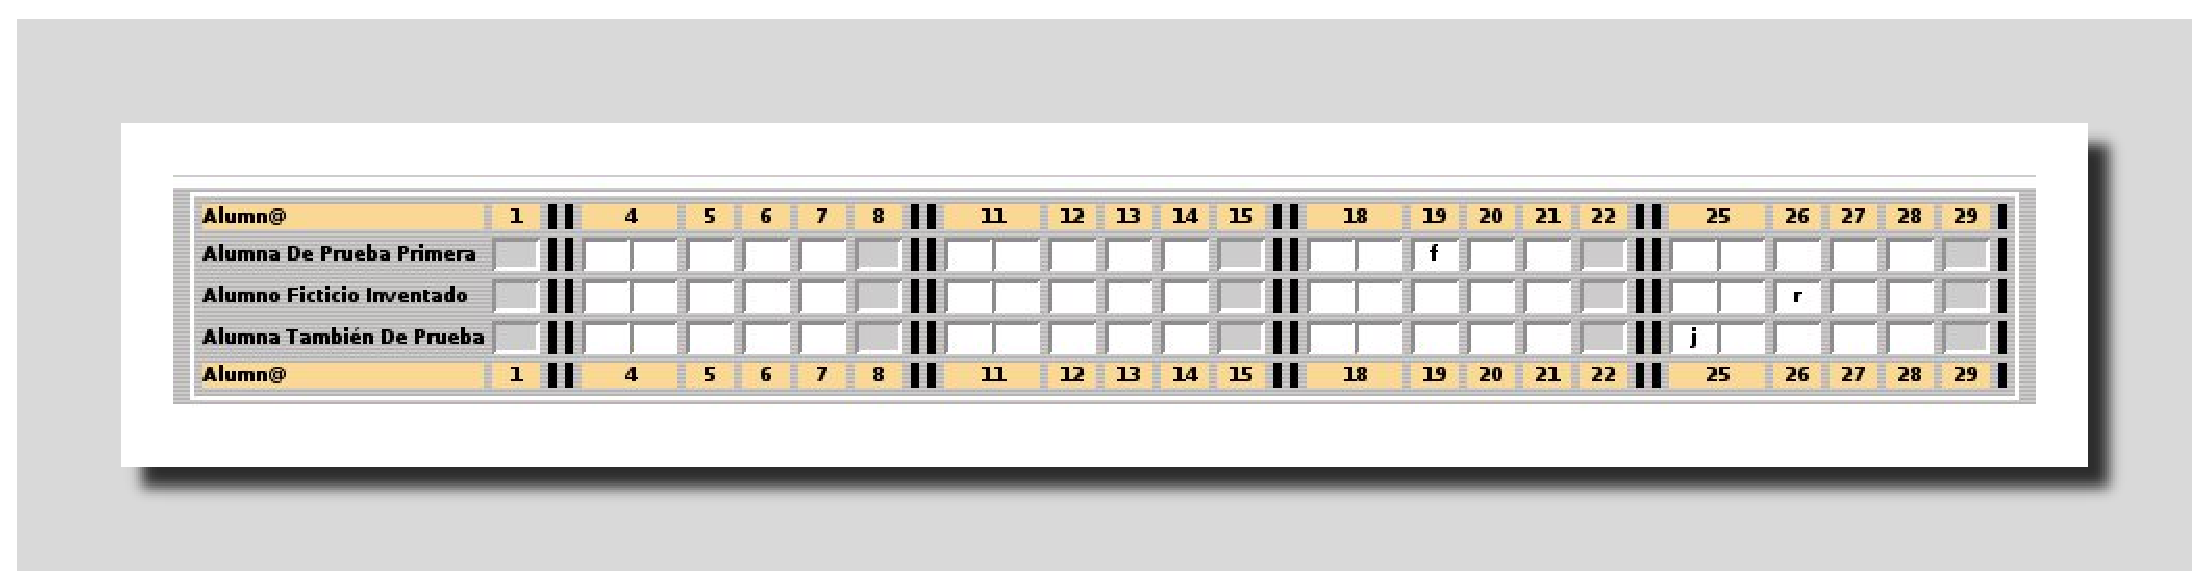
\includegraphics[width=\textwidth]{siestta1.eps}
        \caption{Siestta Attendance Page}
        \label{fig:siestta1}
    \end{center}
\end{figure}

From user point-of-view there are online documentation. This application includes management of students, attendance, marks, tasks, incidents, general queries, letters to parents, interviews with parents, messages, appointments, exams and more.

Several screenshots were taken and their structure will be reused in current application, specially attendance page \ref{fig:siestta1}, and daily schedule \ref{fig:siestta2}.

\begin{figure}
    \begin{center}
        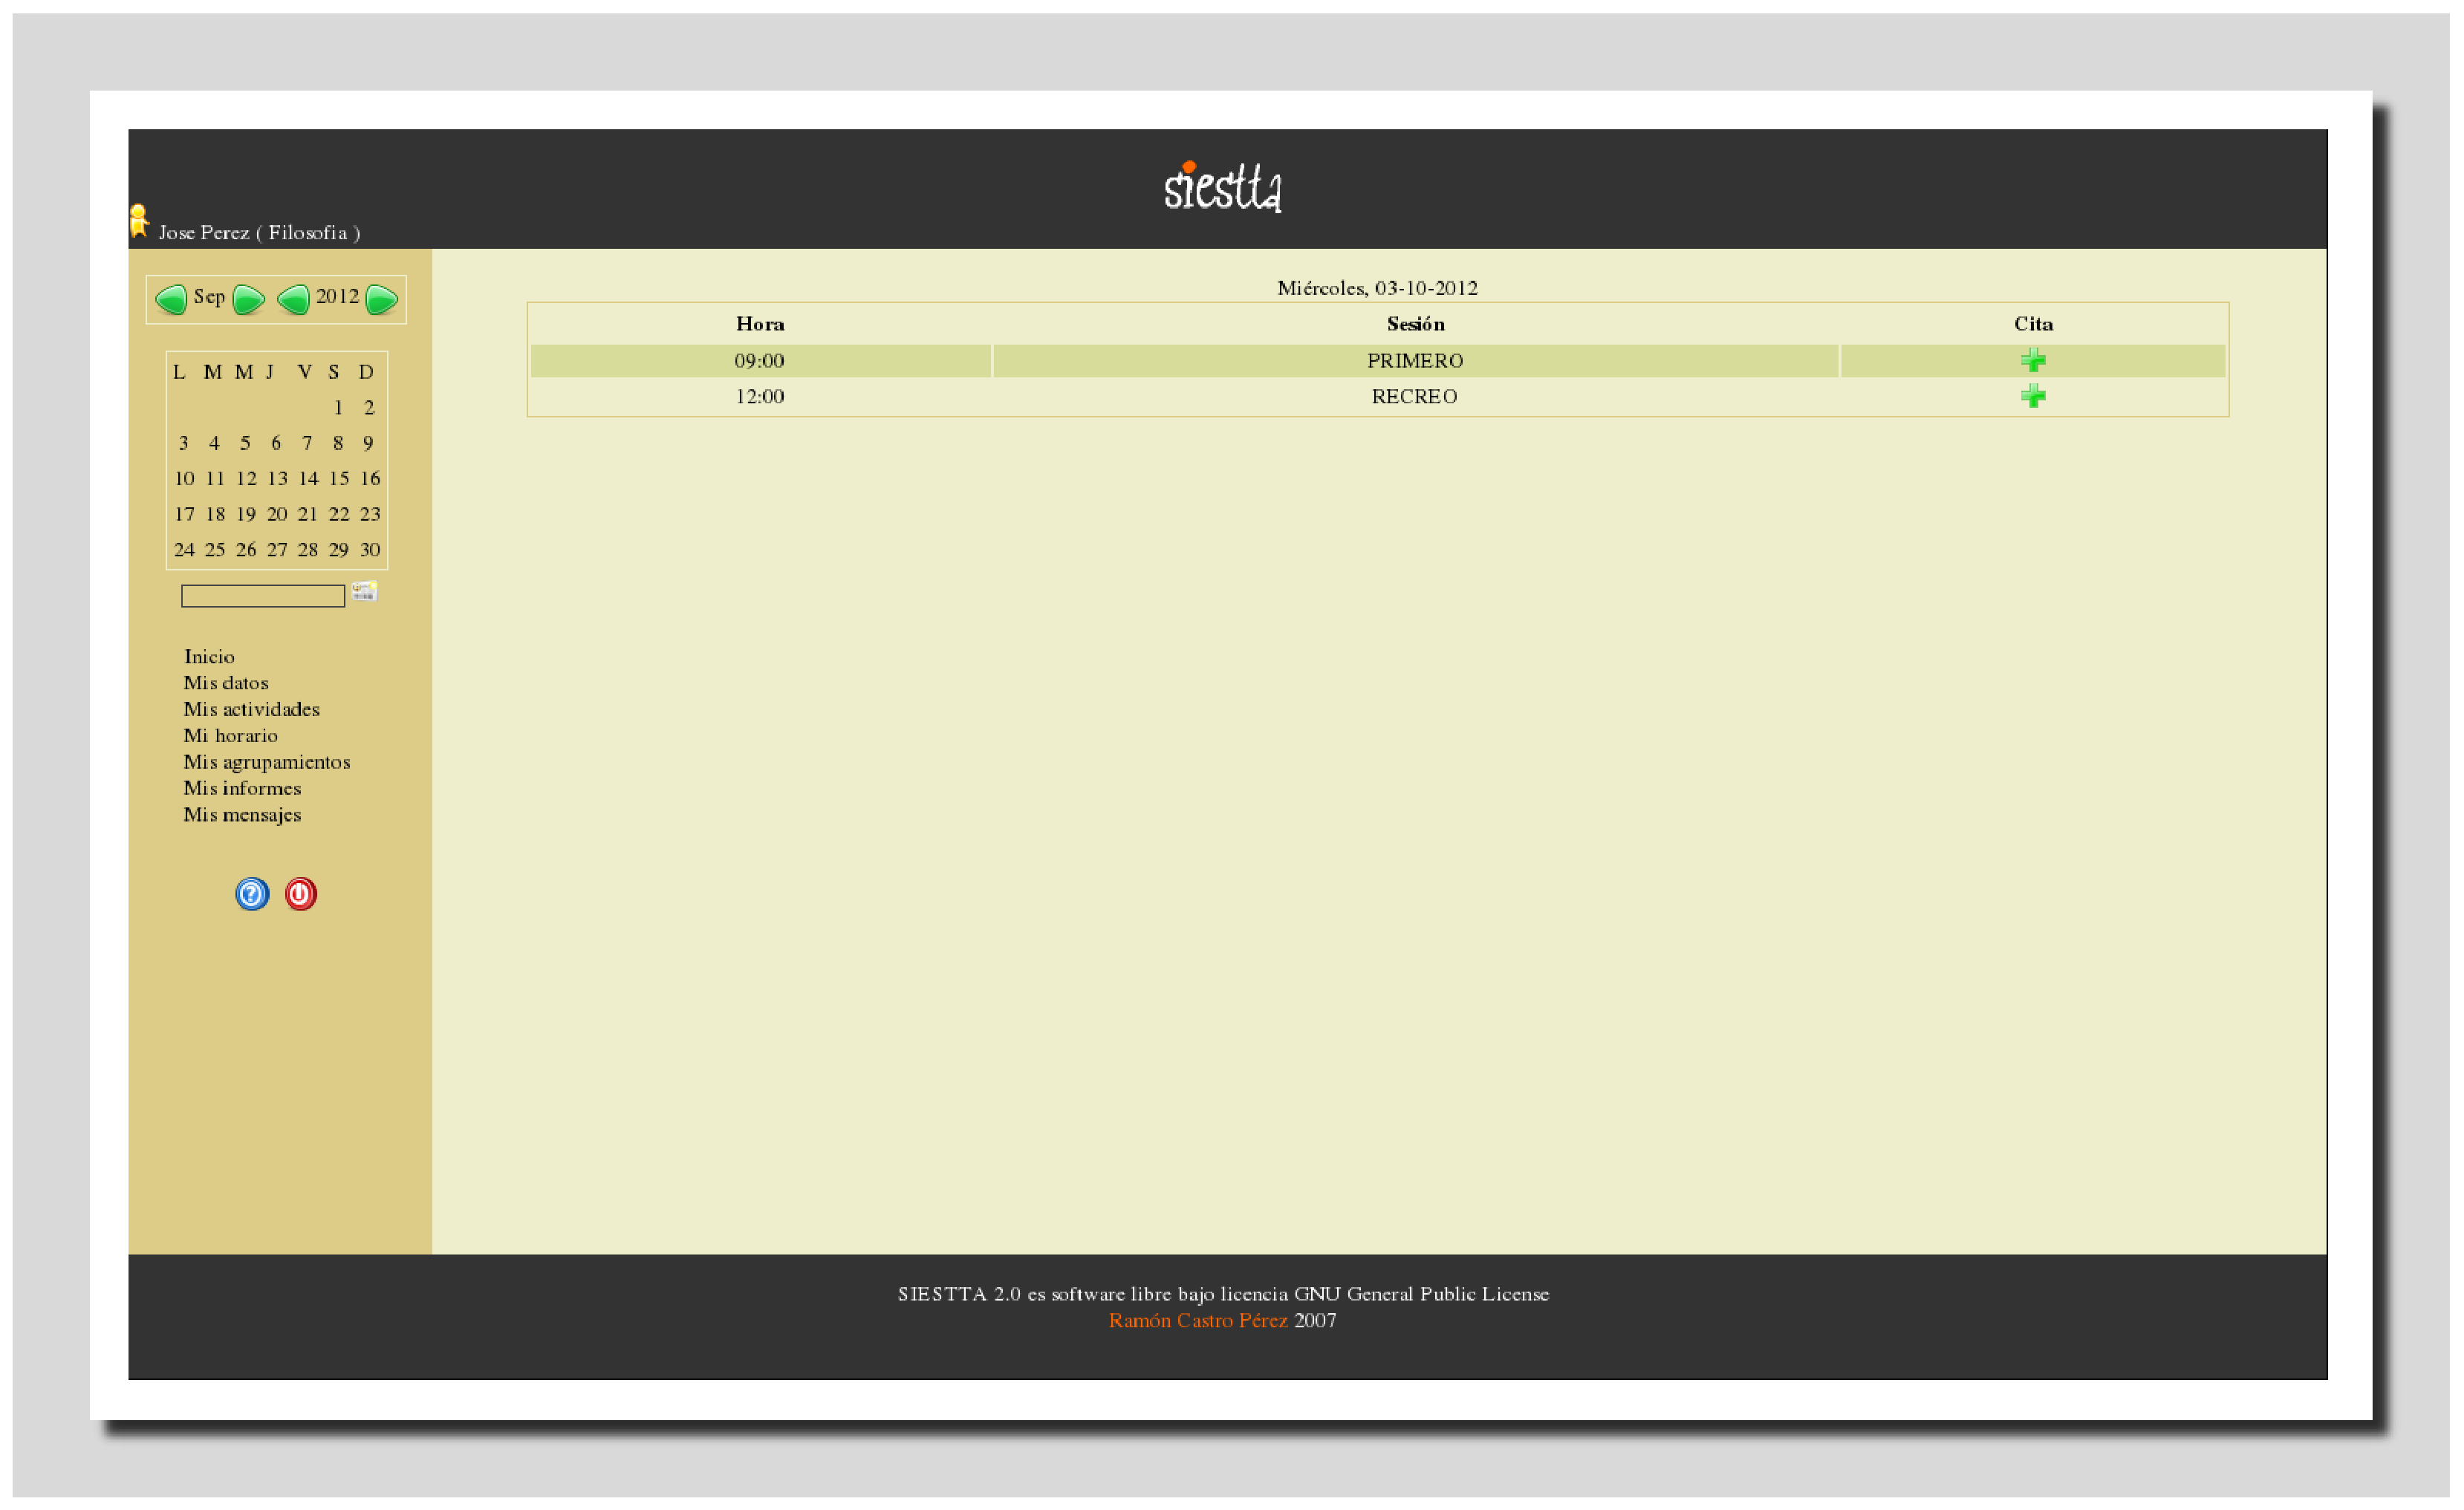
\includegraphics[width=\textwidth]{siestta2.eps}
        \caption{Siestta Main Page}
        \label{fig:siestta2}
    \end{center}
\end{figure}


This application are also available for PDAs, it could be a valid solution but it is server-side with outdated technologies. 
Data structure from Siestta is standard and fully functional, and it will be partially reused by EduXes.\ref{fig:siestta4}.

\begin{figure}
    \begin{center}
        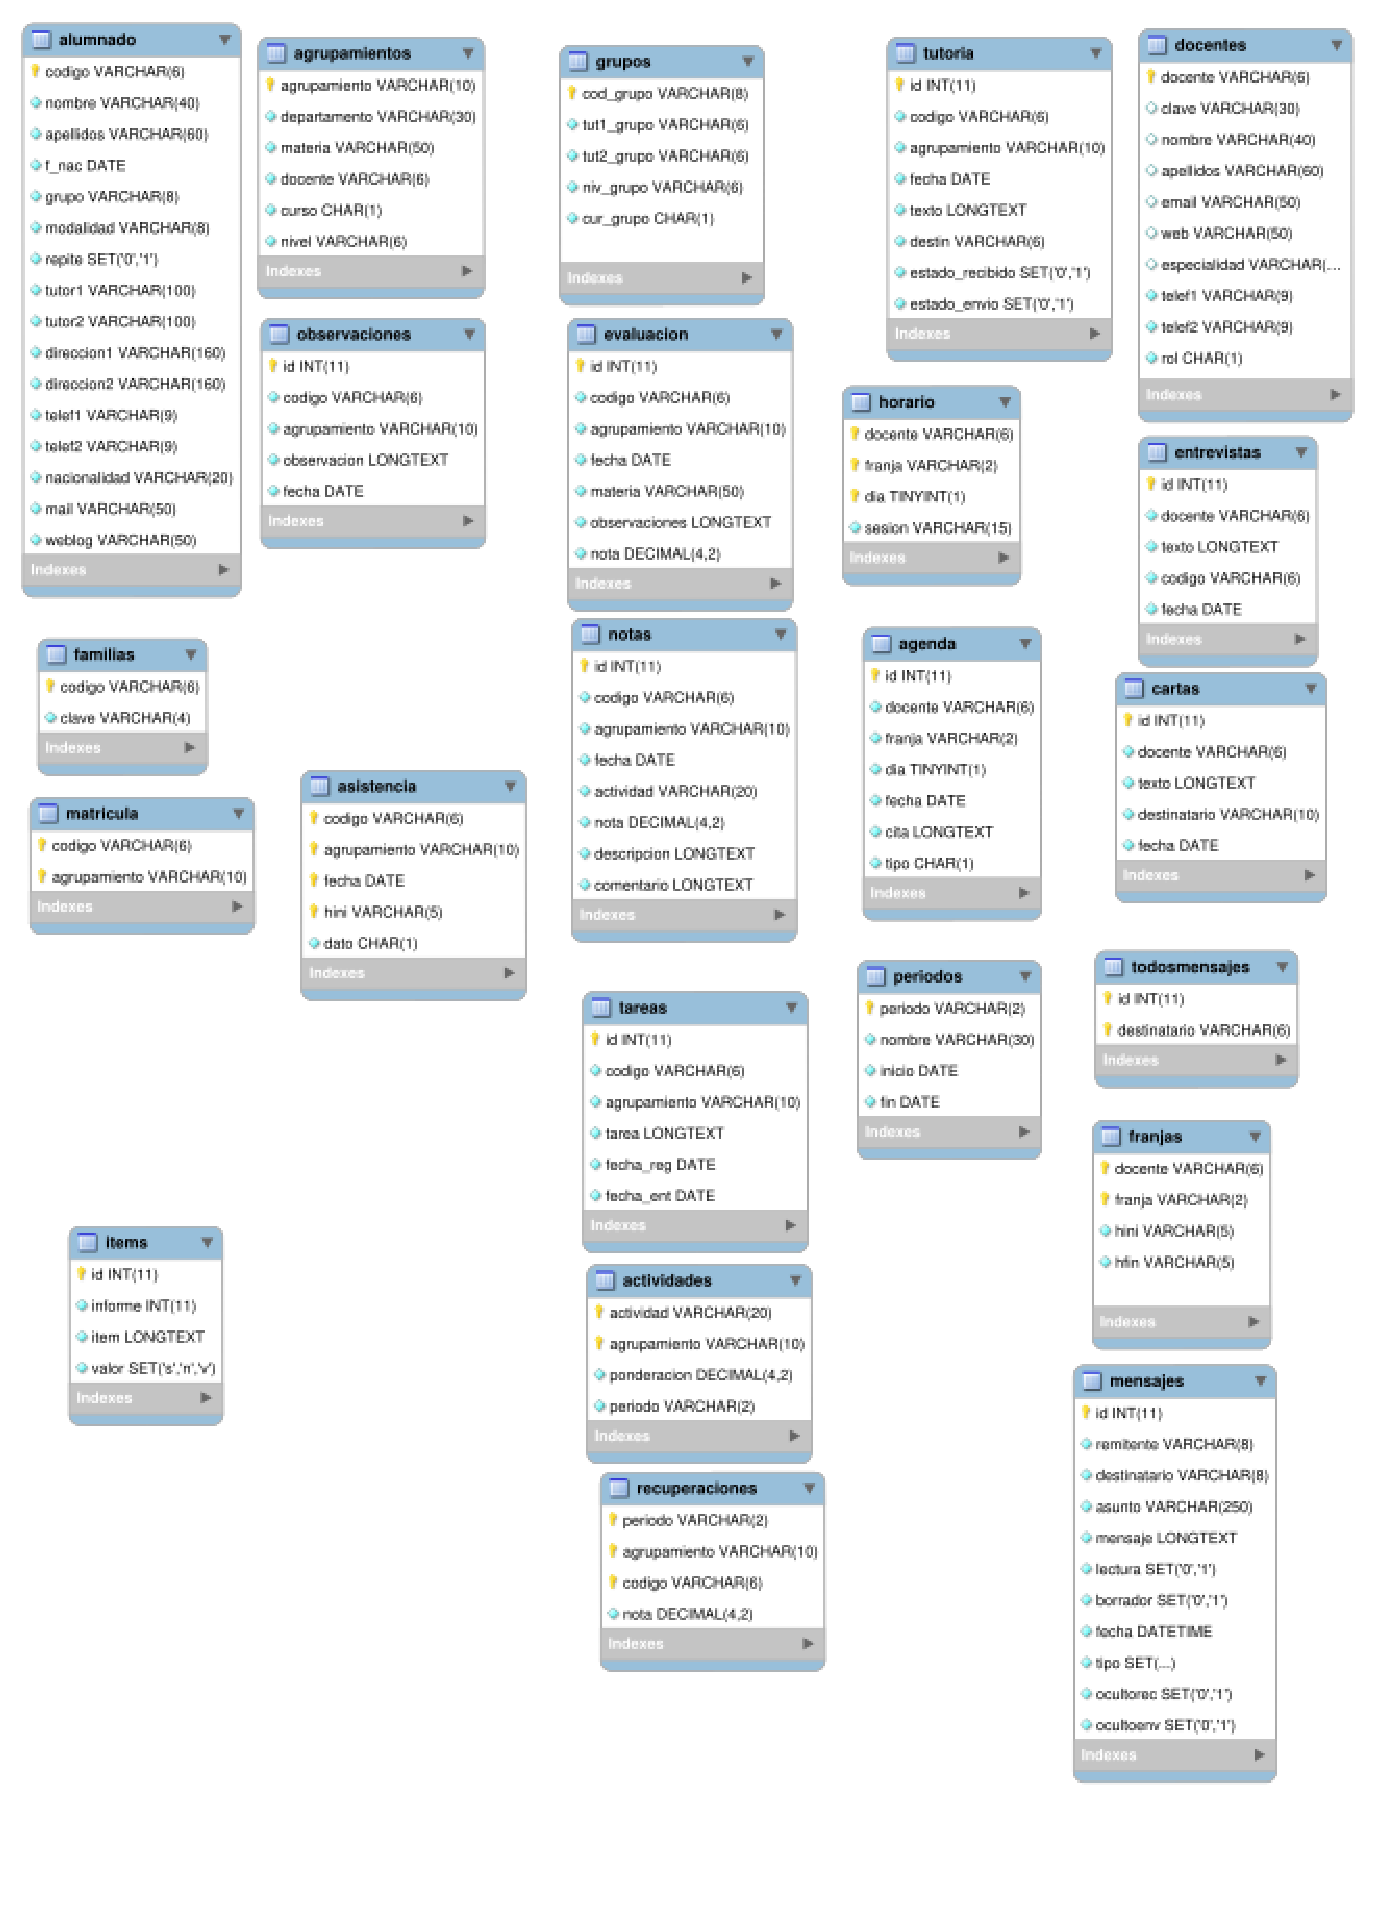
\includegraphics[width=\textwidth]{siestta_sql.eps}
        \caption{Siestta SQL}
        \label{fig:siestta4}
    \end{center}
\end{figure}


Source code are also shown: calendario.php. It shows us a PHP application which uses sessions variables and is not Model-View-Controller oriented.

\begin{bclogo}[couleur=blue!30,arrondi=0.1,ombre=true ] 
{Sample Siestta code: calendario.php}        
        \begin{verbatim}
<?php 
session_start(); 
require('config.php'); 
require('idioma/'.$idioma.''); 
include('funciones_calendario.php'); 
$docente = $_SESSION['usuario_sesion']; 
//recogemos variables 
$mes_actual = $_POST['mes']; 
$anyo_actual = $_POST['anyo']; 
if($mes_actual || $anyo_actual) { 
	include('funciones.php');
	conecta(); 
	}
//si es la primera vez que entramos, cargamos la fecha actual 
if(!isset($mes_actual)) $mes_actual = date('m'); 
if(!isset($anyo_actual)) $anyo_actual = date('Y'); 
//presentamos ahora el calendario del mes actual o cargado 
//tabla con nombre mes y a�o y las flechas para navegar 
echo ' 
<br /> 
<table class="tablacentrada_i"> 
<tr> 
<td> 
<a href="#" onclick="navegaMes(\''.$mes_actual
.'\',\''.$anyo_actual.'\',\'menos\')" title="'.$id_anterior
.'"><img src="imgs/anterior_peq.png" class="alin_bajo" alt="'
.$id_anterior.'" /></a> 
'; 
\end{verbatim}  
\end{bclogo}



\section{Sixa}
Although not GPL'ed, and there are no source code available, several design ideas could be considered: for main page \ref{fig:sixa1},
schedule page \ref{fig:sixa2} and reports page \ref{fig:sixa3}.
\begin{figure}
    \begin{center}
        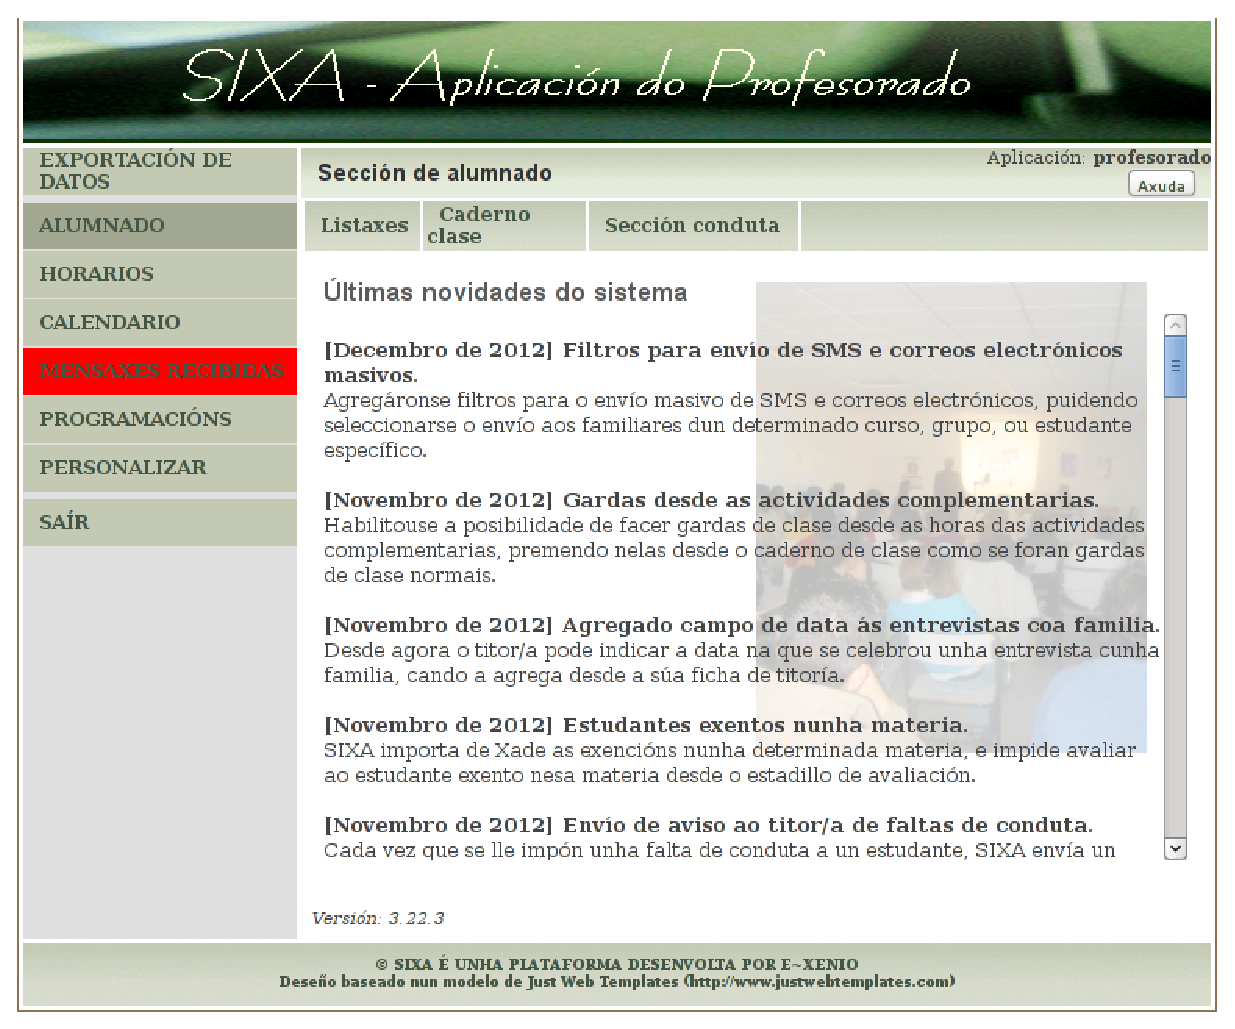
\includegraphics[width=\textwidth]{sixa_1.eps}
        \caption{Sixa Main Page}
        \label{fig:sixa1}
    \end{center}
\end{figure}

\begin{figure}
    \begin{center}
        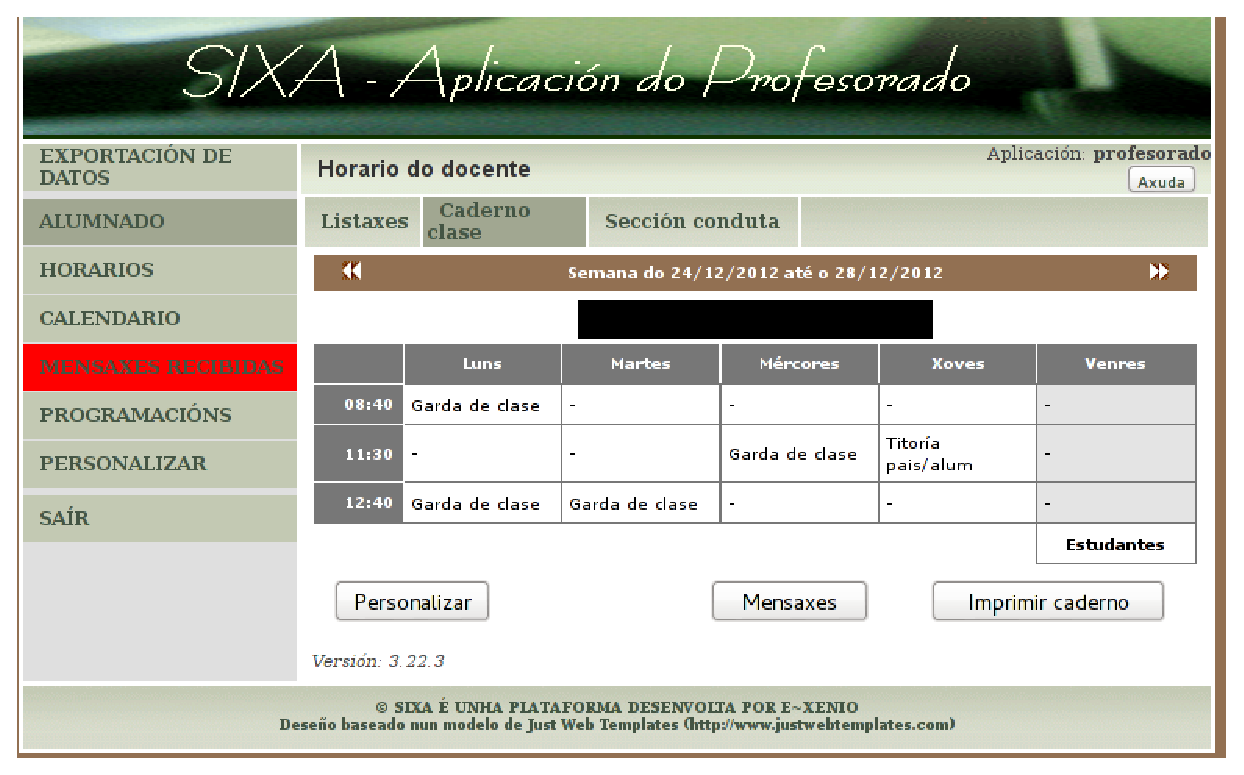
\includegraphics[width=\textwidth]{sixa_2.eps}
        \caption{Sixa Schedule Page}
        \label{fig:sixa2}
    \end{center}
\end{figure}

\begin{figure}
    \begin{center}
        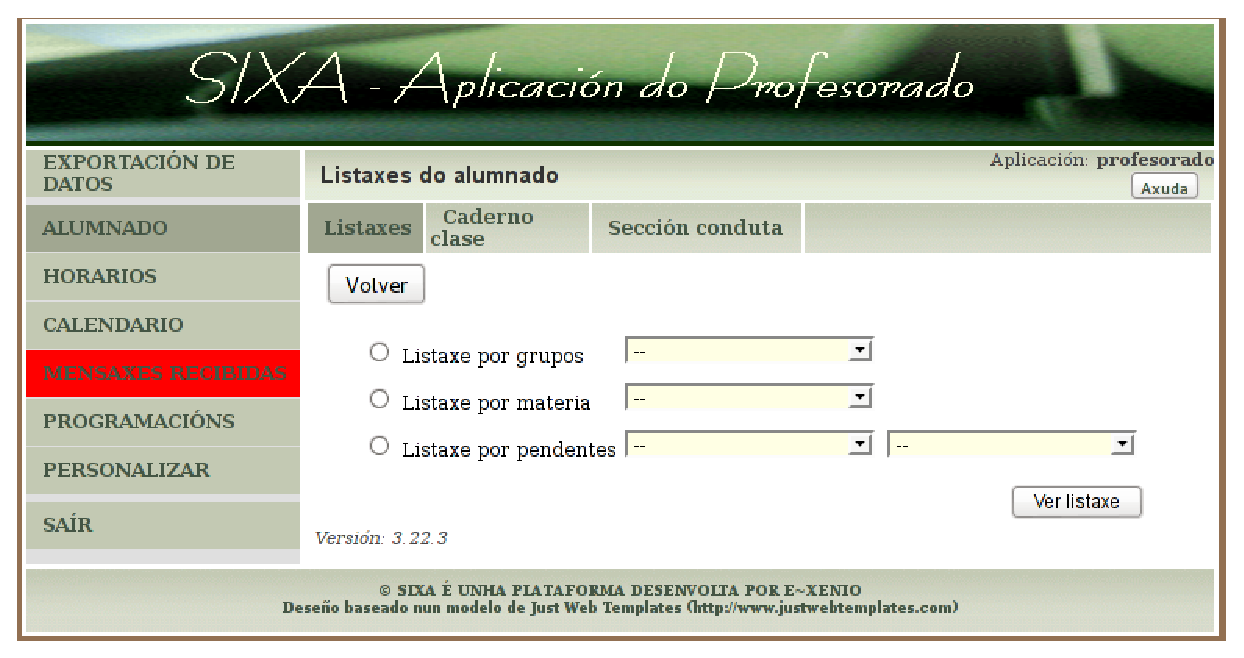
\includegraphics[width=\textwidth]{sixa_3.eps}
        \caption{Sixa Reports Page}
        \label{fig:sixa3}
    \end{center}
\end{figure}
 It has a PDA version (not shown), and it Xade data import capable. Also has a long list of features \cite{Sixa}.


\section{Android applications}
 Several Android applications are listed below, in a short list:

\subsection{Grade Book}
\begin{itemize}
    \item {Name}: Grade Book \cite{Android:Gradebook}
    \item {Description}:Now teachers can manage their students grades directly on their Android device!
    \item {Key Features}:
    \subitem Sync with Google Spreadsheets
    \item {Updated}:July 7, 2011.
    \item {Price }:4 \geneuro
    \item {Screenshot}: \ref{fig:Grade Book}  
\end{itemize}

     
\begin{figure}
    \begin{center}
        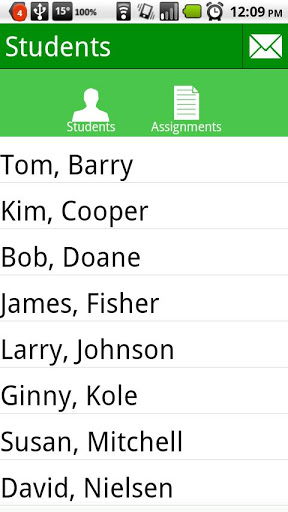
\includegraphics[scale=0.5]{grade_book01.jpg}
        \caption{Grade Book}
        \label{fig:Grade Book}
    \end{center}
\end{figure}

\subsection{Attendance}

\begin{itemize}
    \item {Name}: Attendance \cite{Android:Attendance}
    \item {Description}:Attendance control sync with Google Spreadsheet.
    \item {Key Features}: attendance.
    \item {Updated}:January 13, 2012.
    \item {Price }: Free
        \item {Screenshot}: \ref{fig: Android Attendance}
\end{itemize}


\begin{figure}
    \begin{center}
        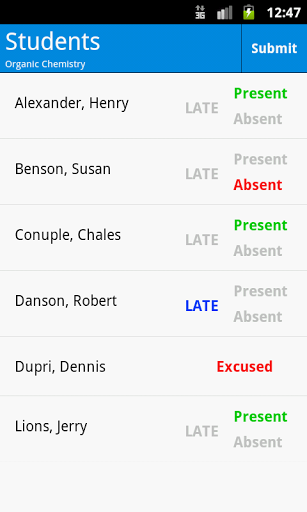
\includegraphics[scale=0.5]{attendance01.png}
        \caption{Attendance}
        \label{fig:Android Attendance}
    \end{center}
\end{figure}




\subsection{Teacher Organizer }
\begin{itemize}
    \item {Name}: Teacher Organizer  \cite{Android:teacherorganizer}
    \item {Description}:Gradebook and attendance, notes, schedule a teacher (high school teacher).
    \item {Key Features}:
    Unified information resource teacher developed within diploma projects.
    \item {Updated}:  December 26, 2012.
    \item {Price }: Free.
      \item {Screenshot}: \ref{fig:TeacherOrganizer}  
\end{itemize}
 It has a drawback: its web page is in Russian, and it is not translated. This application seems to be very professional. There is no code
 avaliable.

\begin{figure}
    \begin{center}
        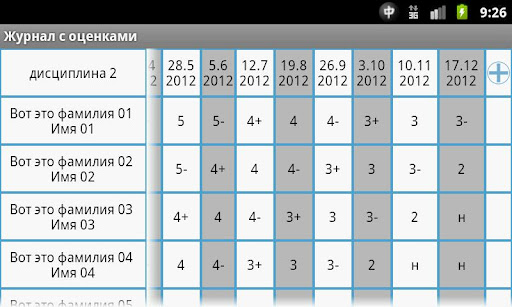
\includegraphics[scale=0.5]{teacher_organizer01.jpg}
        \caption{Teacher Organizer}
        \label{fig:TeacherOrganizer}
    \end{center}
\end{figure}


\subsection{Teacher Aide  }

\begin{itemize}
    \item {Name}: Teacher Aide  \cite{Android:TeacherAide}.
    \item {Description}:The app allows teachers to take attendance and record grades on their phone or tablet.
    \item {Key Features}: Import - export data via CSV. Print via a Google service.
    \item {Updated}: 26 December 2012.
    \item {Price }: Free (Limited number of students).
    \item {Screenshot}: \ref{fig:TeacherAide}  
\end{itemize}

Excellent but not open source or even free.

\begin{figure}
    \begin{center}
        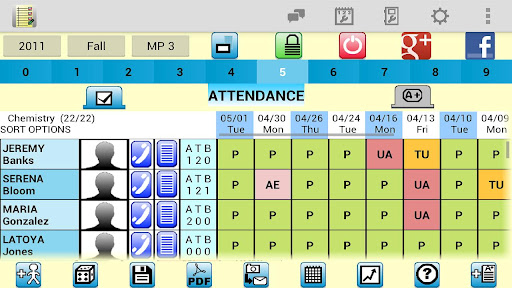
\includegraphics[scale=0.5]{TeacherAideProLite01.jpg}
        \caption{Teacher Aide}
        \label{fig:TeacherAide}
    \end{center}
\end{figure}



% ----------------- OBJETIVO ---------------------------
\chapter {Objetivo (5\%)}

\section {Descripci�n, en un objetivo general, de la finalidad del proyecto.}
\dots
\section {Descripci�n de objetivos parciales que se necesitan cubrir para llegar al objetivo final}
\dots
\section {Descripci�n de alto nivel de las etapas que sigues en el desarrollo}
\dots

% ----------------- DESCRIPCIÓN INFORMÁTICA ------------
\chapter{Description}
 
 A detailed list of procedures to build and prepare environment to develop \emph{EduXes} application, will be described.
 Also a description of how development was carried out, step by step are show.
 

\section{Preparation of development}
Firstly Java Development Kit (JDK) version 1.6 is needed, to build application itself and the Eclipse IDE, is downloaded from \emph{Oracle}: 
\cite{JavaSE}
\begin{quote}
\url{http://www.oracle.com/technetwork/java/javase/downloads/index.html}
\end{quote}

As root user downloaded file is unpacked into {\bf /usr/lib/jvm } and configured to be the Java default:
%%  \begin{bclogo}[couleur=green!30,arrondi=0.1, logo=\bcpanchant,  ombre=true ] 
\begin{bclogo}[couleur=red!30,arrondi=0.1, logo=\bcpanchant,  ombre=true ] 
{Update Java}   
\begin{verbatim}
 # update-java-alternatives -s JDK_1.6_NAME
\end{verbatim}
\end{bclogo}

	\emph{Eclipse Juno (4.6)} is downloaded from its site \cite{Eclipse}: $Download \rightarrow Linux \, 64\, bits$
\begin{quote}
\url{http://www.eclipse.org}
\end{quote}
Android Development Toolkit (ADT)\cite{AndroidDevelopmentKit} is downloaded following instructions on this page:
\begin{quote}
\url{http://developer.android.com/sdk/installing/installing-adt.html}
\end{quote}

	In Eclipse a new line is included into repository software ($Help \rightarrow  Install\, New\, Software \rightarrow Add$):
\begin{quote}
\url{http://dl-ssl.google.com/android/eclipse/}
\end{quote}
	Next step is to select all the related software listed.
	
	For Aptana Plugin the line to be added into Eclipse is: 
\begin{quote}
\url{http://download.aptana.com/studio3/plugin/install}    
\end{quote}

	Furthermore JQuery, JQueryMobile and Phonegap are needed, and were downloaded from their web sites:
	\begin{itemize}
	    \item {JQuery 1.8.1} (no newer versions), from \url{http://jquery.com/} :
	    \subitem JQuery will be  copied into {\bf assets/www/js} folder.
	    \item {JQueryMobile 1.1.1} from \url{ http://jquerymobile.com/}: 
        \subitem JQueryMobile is a zip file which will be uncompressed and copied into  {\bf assets/www/js} folder.
        \item{PhoneGap - Cordova 1.8.1} is downloaded from \url{https://github.com/phonegap/phonegap/zipball/1.8.1}
        and installed following reference \cite{PhoneGapGS} 

	\end{itemize}

	To create a PhoneGap application there are very important instructions (Getting Started with Android)  should be followed step by step:
\cite{AndroidGettingStarted}
\section{Application Skeleton}
  Next step is to choose application name and folders policy. Name \emph{EduXes} stands for "Educaci\'n" and "Xesti\'on", is a educational management software.
About folders policy, a folder is created ({\bf assets/www/js}) which contains javascript ({\bf *.js}) files except \emph{JQuery} and \emph{JQueryMobile} which is included into another
 folder ({ \bf assets/www/js/jquery} ), do not forget style sheets files ({\bf *.css } )
 
To finish building application skeleton a simple application is created which contains only a blank page.
 
Getting started with Android \cite{AndroidGettingStarted} is followed step by step.

\section{Upload into Git repository}

 Following stage is to upload that simple application into a git repository. 
An account is created in Github\cite{GitHub}, which is the largest code host in the world,  and a new application is initialized.  This are the source code project page \url{https://github.com/joseantoniosa/EduXes}.

Then source code are upload to Github: 

  \begin{bclogo}[couleur=green!30,arrondi=0.1, logo=\bcpanchant,  ombre=true ] 
{Git init shell}   
\begin{verbatim}
$ git init
$ git add -A *
$ git remote add  EduXes git@github.com:joseantoniosa/EduXes.git 
$ git push origin master
\end{verbatim}
\end{bclogo}

Each time an update in code is done,  code is uploaded :

  \begin{bclogo}[couleur=green!30,arrondi=0.1, logo=\bcpanchant,  ombre=true ] 
{Git update}   
\begin{verbatim}
$ git add -A *
$ git commit -m 'CHANGES_DESCRIPTION'
$ git push origin master
\end{verbatim}
\end{bclogo}


\section{Development}
 Before begining with development itself is compulsory to explain some concepts already shown above in Methodology (\ref{Methodology}), but with more detail:
JQueryMobile \cite{JQueryMobile} and by extension,  PhoneGap \cite{PhoneGap}  applications, are structured in pages:
 \begin{quote}
  <div data-role="page">
 \end{quote}

   which are very similar to desktop applications windows. Therefore, from Javascript code, to change to a new page 
\begin{quote}
 \$.mobile.changePage("\#daily\_work");
\end{quote}
       opens \textit{"daily\_work"} page.  
     
% Application Work-flow 
% Next illustration try to be self-explicative.  Beginning at onDeviceReady()  from interface.fs file.  Inside each page several actions are performed: e.g., open and populate database, load list of groups (loadSchedule()),  and user choose next step according options shown. 
% 
% 
% %%%%%%%%%%%%%%%%%%%%%%%%%%%%%%%%%
% 
% 
% Development:
As shown before (\ref{Methodology}) \emph{EduXes} contains several files:
\begin{itemize}
\item Four files contain application code:
\subitem  {\bf interface.js} : It contains information and decisions related to interface and application workflow, completely independent from database. It is located in {\bf assets/www/js} folder.
\subitem { \bf database.js} : It contains database related code: SELECT, INSERT, etc. It is located in {\bf assets/www/js} folder.
\subitem {\bf index.html}, {\bf remove.html} only contain HTML framework, page properties, and static content.  They are located in {\bf assets/www/} folder.
\item There are three important files which contain documentation:
\subitem {\bf TODO.txt}. List of goals to be achieved and milestone reached. It is located in root application folder.
\subitem {\bf DATABASE.sql}.  Data-base structure in SQL format. This file are shown below. It is located in root application folder.
\subitem {\bf REAME.txt}. Only contains general information about this application.It is located in root application folder.
\end{itemize}

Also, \emph{Eclipse} generates several files, the most important is the application file, which is an {\bf apk } package: {\bf bin/EduXes.apk}.

Next step is to build database, this will be described below \ref{DataBase}. 
Following database, sample data is needed to begin application development. 
\subsection{Groups}

The first window to be developed is \emph{List of Groups}: as shown above \ref{Methodology}, firstly a \emph{page} is created inside {\bf index.html}. This page, as every page,  has three important elements:
\begin{itemize}
    \item  \emph{header}. It could contain a backward button, which return application flow to previous visited page. This is disabled,
because it could cause problems when previous page is an edit page, and another solution is preferred.    
    \item \emph{content}. Data itself, it has an important \emph{id} to be filled with content by javascript code.
    \item \emph{footer}. Usually page name.
\end{itemize}

\begin{figure}
    \begin{center}
        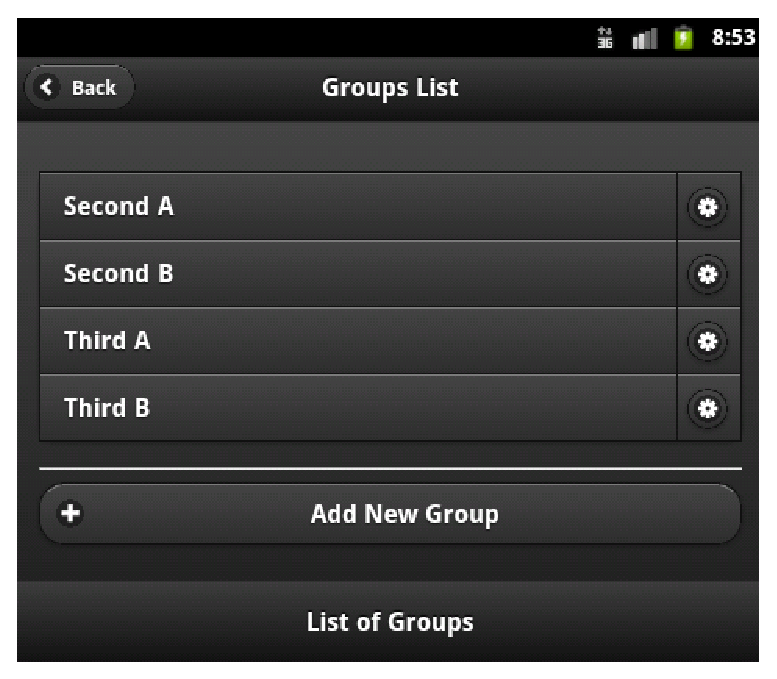
\includegraphics[width=\textwidth]{eduxes_groups_list.eps}
        \caption{Groups}
        \label{fig:EduXesGroups}
    \end{center}
\end{figure}



\begin{bclogo}[couleur=blue!30,arrondi=0.1,ombre=true ] 
%% \begin{bclogo}[couleur=blue!30,arrondi=0.1, logo=\bcpanchant, barre=zigzag,  ombre=true ] 
{List Groups page. index.html}
\begin{verbatim}
<div data-role="page" id="list_groups" data-add-back-btn="true">
    <div data-role="header"  data-add-back-btn="false"  >
        <a href="#list_settings"  data-icon="arrow-l"
             data-theme="a" data-role="button">Back</a>
        <h1>Groups List</h1>
    </div>                
    
    <div data-role="content">
    <ul id="groups_ul" data-role="listview" data-inset="true"  
        data-split-icon="gear" data-split-theme="a" >
    </ul>
     <hr />
     <a  style="text-align: center" onClick="onAddNewGroup();" 
        data-role="button" data-icon="add">Add New Group</a>
    </div>
    <div data-role="footer"  data-rel="back" data-theme="a">
     <p style="text-align: center">List of Groups</p>
    </div>
</div>
\end{verbatim}
\end{bclogo}
To fill this list of elements \emph{<ul id=groups\_ul (...)>} a function \emph{onListAllGroups()} is called. Firstly a
\texttt{loading ...} logo appears, then a function from {\bf database.js} is called (\emph{loadAllGroups() }).
\begin{bclogo}[couleur=blue!30,arrondi=0.1,ombre=true ] 
{List Group page. interface.js}
\begin{verbatim}
function onListAllGroups(){
    $.mobile.showPageLoadingMsg();
    table_global='GROUPS';
    loadAllGroups(global_db); // #groups_ul
    $.mobile.changePage("#list_groups", { transition: "slideup"} );
}
\end{verbatim}
\end{bclogo}

Function (\emph{loadAllGroups() }) calls (\emph{queryAllGroupsDB()}) from \texttt{database.js}. 
This function fills \textit{\$('\#groups\_ul')}  combo box with group data: \textit{name}. Moreover user
can access  a list of students of that group (\textit{listStudentsByGroup()}) or change
group information (\textit{EditGroup()}).


\begin{bclogo}[couleur=blue!30,arrondi=0.1,ombre=true ] 
{List Group page. database.js}
\begin{verbatim}
function queryAllGroupsDB(tx) {
    log("Query All Groups \n");
    var ul_list =$('#groups_ul');
    tx.executeSql('SELECT * FROM GROUPS', [],
        dbSuccessFunc = function(tx, rs) {
        ul_list.empty();
        var html ="";
        for (var i = 0; i < rs.rows.length; i++) {
          id = rs.rows.item(i).id ;
          html = "<li>";
          html += "<a onClick='global_id=" + id + 
              "; global_id_group="+id
              +"; table_global=\"groups\"; ";
          html += " listStudentsByGroup(" + id + " );'  ";
          html += " href='#' >";
          html += rs.rows.item(i).data;
          html += "</a>";
          html += " <a data-role='button' data-position-to='window'";
          html += " data-iconpos='notext' ";
          html += " style='float:right;' href='#' ";
          html += " data-rel='dialog' data-theme='a' ";
          html += " data-transition='slideup' ";
          html += " onClick=\"EditGroup(" + id + "); ";
          html += " global_id_group="+id
              +"; global_id=" + id + "; \">Edit</a>";
          html +="</li>";
          ul_list.append(html);
        }
        ul_list.listview('refresh'); },
        dbErrorFunc = function(ttx, e) {
            if (ttx.message)
                e = ttx;
            log(" There has been an error Select * from groups : " 
            + e.message);
        return false;
    });
}
\end{verbatim}
\end{bclogo}


Second window to be developed is edit group information. The contents of \textit{Edit Group} page from \textbf{index.html} is
filled by loadGroup() function \textbf{database.js} as shown below \ref{edit_group_database}.

\begin{bclogo}[couleur=blue!30,arrondi=0.1,ombre=true ] 
{Edit Group page. index.html }
\begin{verbatim}
<div data-role="page" id="edit_groups" data-add-back-btn="true">
    <div data-role="header"  data-add-back-btn="true" >
        <h1>Group Edition</h1>
    </div>
    <div data-role="content">
        <label for="nombre_grupo">Name</label>
        <input id="in_nombre_grupo" enabled="true" />
        <label for="nivel_grupo">Level</label>
        <input id="in_nivel_grupo" enabled="true" />
        <a onClick="onUpdateGroup();" data-role="button" 
            data-icon="check">Save</a>
	</div>
</div>
\end{verbatim}
\end{bclogo}



\begin{bclogo}[couleur=blue!30,arrondi=0.1,ombre=true ] 
{Edit Group page. interface.js}
\begin{verbatim}
function EditGroup(id_group){
    $.mobile.showPageLoadingMsg();
    global_id = id_group;      //local variable goes global
    table_global = 'GROUPS';
    loadGroup(global_db,id_group);
    $.mobile.changePage("#edit_groups", { transition: "slideup"});
}
\end{verbatim}
\end{bclogo}

Inside \textit{loadGroup} function a sql query is built \texttt{(SELECT ... FROM ...)}, then
it is executed and returned values are loaded in result set variable (\textit{rs}). 
With this data html form  is populated (\textit{\$('\#in\_nombre\_grupo')}). 
Whether an error is triggered then \textit{dbErrorFunc} is called an a message appears on user interface.

These procedure will be very similar to all \textit{"load"} functions (students, activities).

\begin{bclogo}[couleur=blue!30,arrondi=0.1,ombre=true ] 
{Load Group page. database.js  \label{edit_group_database}}
\begin{verbatim}
function loadGroup(db, id_group){
    db.transaction(function (tx) {
        log("Query Group \n");
        var sql = 'SELECT id, data, other_data ':
        sql += ' FROM GROUPS WHERE id ='+id_group;
        tx.executeSql(sql, [],
            dbSuccessFunc = function(ttx,rs){
                $('#in_nombre_grupo').val(rs.rows.item(0).data);
                $('#in_nivel_grupo').val(rs.rows.item(0).other_data);
            },
            dbErrorFunc = function(tx, e) {
                if (tx.message) e = tx;
                    log(" There has been an error queryGroupDB: " 
                        + e.message);
                    alert(" There has been an error queryGroupDB: " 
                        + e.message);
                    return false;
            });
    });
}
\end{verbatim}
\end{bclogo}


\subsection{Students}    

Students pages are very similar to groups but, of course, they contain different fields (a complete list of fields is shown in database
definition \ref{DataBase}). Only list of students by group page and \textit{LoadStudentsByGroup} code are shown. 
They are very similar to their \textit{groups} counterpart. The main concern is about escape characters and colons,
code is straightforward to read. Several lines were removed towards readability (...). 

\begin{figure}
    \begin{center}
        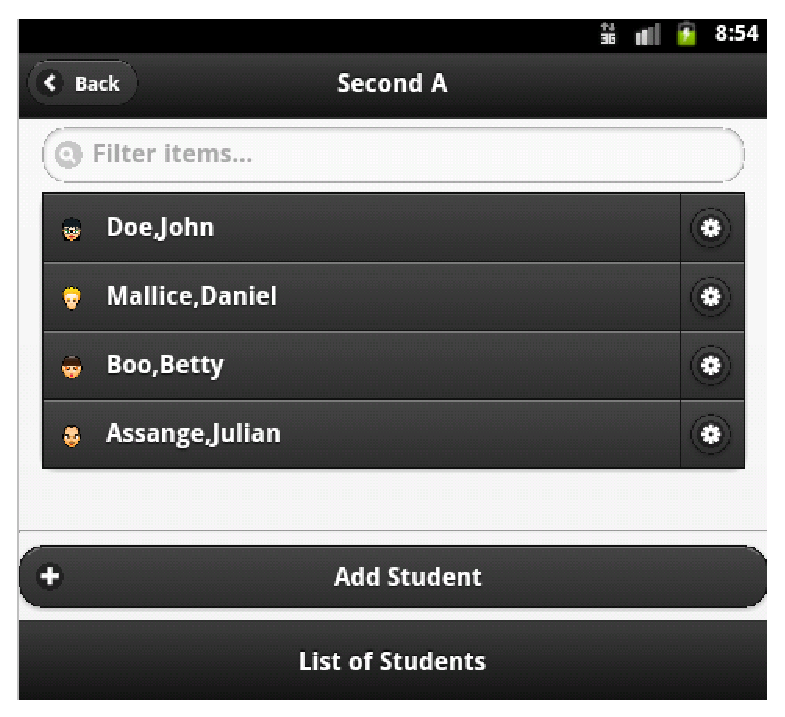
\includegraphics[width=\textwidth]{eduxes_list_students.eps}
        \caption{Students}
        \label{fig:EduXesStudents}
    \end{center}
\end{figure}



\begin{bclogo}[couleur=blue!30,arrondi=0.1,ombre=true ] 
{List Students page. index.html \label{list_students_page}}
\begin{verbatim}
<div data-role="page" id="list_students_by_group" 
    data-add-back-btn="true">
    <div data-role="header"  data-back-btn-text="previous" 
        data-add-back-btn="true" >
        <h1 id="id_list_students_by_group"> Students List</h1>
    </div>
    <div data-role="content">
        <ul id="list_students_by_group_ul" data-role="listview" 
        data-theme="a" data-split-theme="a" data-split-icon="gear" 
        data-filter="true" data-inset="true"  >
        </ul>
    </div>
    <hr />
    <a onClick="onAddNewStudent();" data-role="button" 
    data-icon="add"  data-theme="a" >Add Student</a>
    <div data-role="footer" class="footer-docs" data-rel="back" 
    data-theme="a">
        <p style="text-align: center">
            List of Students
        </p>
    </div>
</div>
\end{verbatim}
\end{bclogo}


\newpage


\begin{bclogo}[couleur=blue!30,arrondi=0.1,ombre=true ] 
{Load Student snippet. database.js  \label{load_student_database}}
\begin{verbatim}
function loadStudentsByGroup(db,id_group) {
 db.transaction(
  function (tx) {
   var sql = 'SELECT STUDENTS.id as id, ';
   sql += ' STUDENTS.id_group as id_group,';
   sql += ' STUDENTS.name as name, ';
   (...)
   sql += ' FROM STUDENTS, GROUPS WHERE ';
   sql += ' STUDENTS.id_group = g_id AND id_group=';
   sql += ' + id_group;
   tx.executeSql(sql, [],
    dbSuccessFunc = function(tx, results) {
     var len = results.rows.length;
     var ul_list = $('#list_students_by_group_ul');
     $('#id_list_students_by_group').text(
        results.rows.item(0).data );
     var html;
     ul_list.empty();
     var id = 0;
     for (var i = 0; i < len; i++) {
        id = results.rows.item(i).id;
        html="<li >";
        html+="<a onClick='global_id="+id;
        html+=";table_global=\"students\";'"; 
        html+=" href='#' data-rel='dialog' ";
        html+=" data-transition='slideup'>";
(...)
        html+=results.rows.item(i).surname + "," ;
        html+=results.rows.item(i).name+"</a>";
        html+="<a data-role='button' "; 
        html+=" data-position-to='window' ";
        html+=" data-iconpos='notext' "; 
        html+=" style='float:right;' href='#' ";
        html+=" data-rel='dialog' ";
        html+=" data-transition='slideup'  ";
        html+=" onClick=\"EditStudent(" ;
        html+=id + ");\">Edit</a> </li>";
        ul_list.append(html);
    }
    ul_list.listview('refresh'); },
    dbErrorFunc = function(tx, e) {
     if (tx.message) e = tx;
     log(sql);
     log(" Error loadStudentsByGroup: "+e.message);
     alert("Error loadStudentsByGroup: " + e.message);
     return false;
    });
    }
   );
}
\end{verbatim}
\end{bclogo}

\subsection{Main Page}

Main page was not the very first page to be built, because it is related with attendance, sessions, groups and students, and also reports.
Its design it has to follow several basic principles: simple but with no more than four clicks (even less)away to 
 access to every application window-page. The most important item is current data, and the \textit{">" } symbol on the right to access \textit{Attendance} page.
 
 There are a table with three columns (\textit{class="ui-grid-b"}), which contains a label, the current date, and an info button.
 An a list of navigation buttons to list data (\texttt{report}) or manage students, groups and activities (\texttt{settings})
 
Of course there are a lot of elements that could be changed to improve user experience in this page.

\begin{figure}
    \begin{center}
        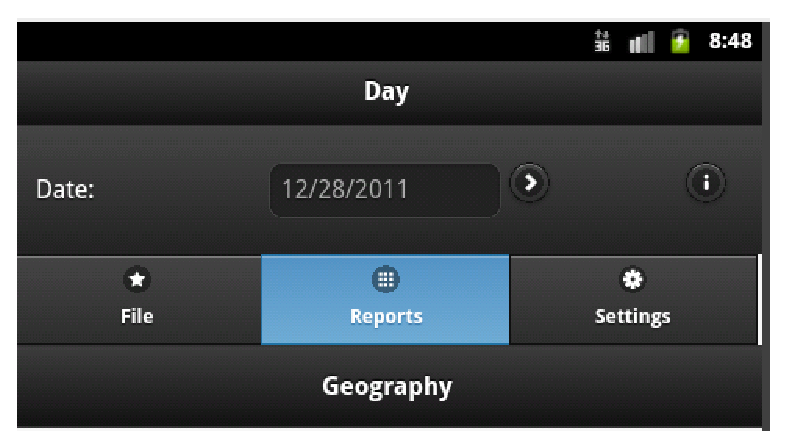
\includegraphics[width=\textwidth]{eduxes_main_page1.eps}
        \caption{Main Page}
        \label{fig:EduXesMainPage}
    \end{center}
\end{figure}


\begin{bclogo}[couleur=blue!30,arrondi=0.1,ombre=true ] 
{Main Page. index.html \label{main_page}}
\begin{verbatim}
<!-- Main Window    //-->
<div data-role="page" id="daily_work">
    <div data-role="header" data-add-back-btn="true" data-theme="a">
        <h1>Day</h1>
    </div>
    <div data-role="content" data-theme="a">
        <div class="ui-grid-b">
        <div class="ui-block-a">
            <div data-role="fieldcontain">
                <label for="date"  >Date:</label>
            </div>
        </div>
        <div class="ui-block-b">
            <input id="daily_date_scroller" 
            name="daily_date_scroller" />
        </div>
        <div class="ui-block-c">
            <a href="#" data-role='button' 
            data-icon='info' data-iconpos='notext' 
            style='float:right;' onClick="help('date');">Help</a>
            <a href="#" data-role="button" 
            data-icon="arrow-r" data-iconpos="notext"  
            onClick="open_daily_page() " >Go</a>
        </div>
    </div>
    </div>
    <div data-role="navbar">
        <ul>
            <li>
                <a href="#" onClick="onGeneralFile()  "  
                data-role="button" data-icon="star"  
                data-theme="a" > File</a>
            </li>
            <li>
                <a href="#" onClick="onGeneralListReports();"  
                data-role="button" data-icon="grid"  
                data-theme="a" >Reports</a>
            </li>
            <li>
                <a href="#" onClick="onGeneralListSettings();" 
                data-role="button" data-icon="gear"   
                data-theme="a" >Settings</a>
            </li>
        </ul>
    </div><!-- /navbar -->
    <div data-role="footer" class="footer-docs" data-theme="a">
        <p   style="text-align:center;"  id="teachers_name"></p>
    </div>
</div>
\end{verbatim}
\end{bclogo}


\subsection{Attendance}

\begin{figure}
    \begin{center}
        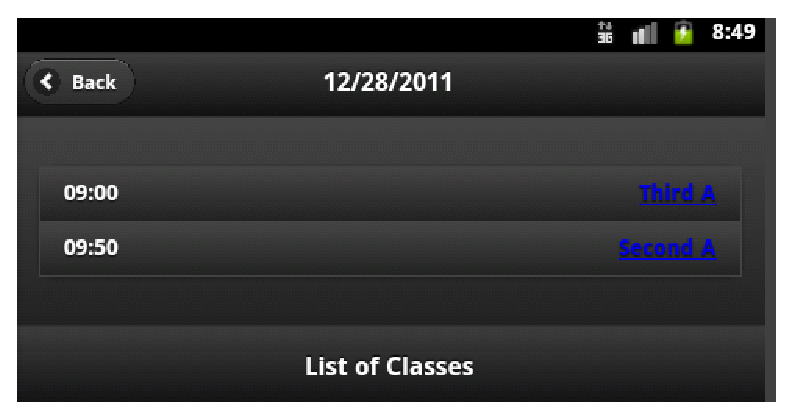
\includegraphics[width=\textwidth]{eduxes_schedule1.eps}
        \caption{Schedule}
        \label{fig:EduXesSchedule}
    \end{center}
\end{figure}




\texttt{Attendance} per group is one of most important pages, and it list attendance, behaviour of 
students of a group. There is a previous page: list of groups for current day (\textit{Schedule page})
(Figure: \ref{fig:EduXesSchedule}) \ref{schedule_page}.

\begin{bclogo}[couleur=blue!30,arrondi=0.1,ombre=true ] 
{Schedule Page. index.html \label{schedule_page}}
\begin{verbatim}
<div data-role="page" id="daily_schedule"  
 data-add-back-btn="false"  data-theme="a" >
    <div data-role="header"  
        data-back-btn-text="previous" 
        data-add-back-btn="false" data-theme="a">
        <a href="#daily_work"  
        data-icon="arrow-l" data-theme="a" 
        data-role="button">Back</a>
        <h1 id="current_day"> Current Day</h1>
    </div>
    <div data-role="content" data-theme="a">
        <ul id="groups_day_ul" data-role="listview" 
        data-inset="true" data-split-icon="gear"  
        data-split-theme="a" >
        </ul>
    </div>
    <div data-role="footer" class="footer-docs" 
        data-add-back-btn="true" data-theme="a">
        <p  style="text-align:center;" > List of Classes</p>
    </div>
</div>
\end{verbatim}
\end{bclogo}

\begin{figure}
    \begin{center}
        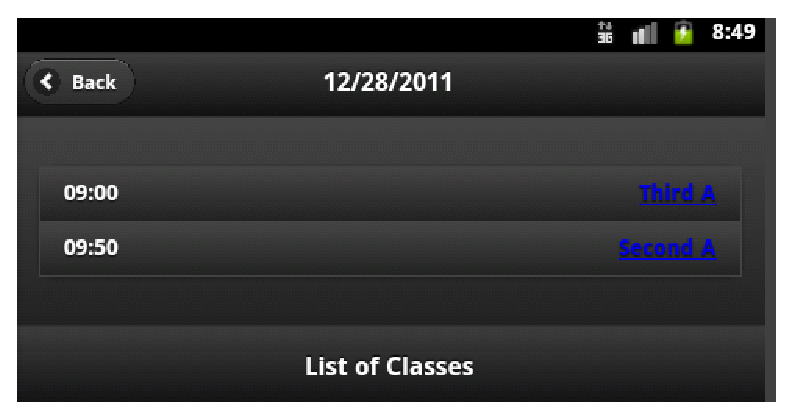
\includegraphics[width=\textwidth]{eduxes_schedule1.eps}
        \caption{Attendance}
        \label{fig:EduXesAttendance}
    \end{center}
\end{figure}

The \textit{queryStudentsAttendanceSuccess} \ref{attendance_student} function fills \textit{Attendance} page \ref{attendance_page} with photos, names and surnames
of student of the adequate group. User can choose among different student "states", these "states" are filled in
\textit{fillSelectStudent} function. When user changes combo values function \textit{studentState} is called which
update or insert student state into \textit{attendance} table in database.

\begin{bclogo}[couleur=blue!30,arrondi=0.1,ombre=true ] 
{Attendance Page. index.html \label{attendance_page}}
\begin{verbatim}
<div data-role="page" id="list_students_attendance" 
    data-add-back-btn="false">
    <div data-role="header"  data-back-btn-text="previous" 
        data-add-back-btn="false"  data-theme="a" >
        <a href="#" onClick="open_daily_page();" data-icon="arrow-l" 
            data-theme="a" data-role="button">Back</a>
        <h1 id="current_group_attendance">Student List for Group</h1>
    </div>
    <div data-role="content"> <!---Data goes here //-->
        <ul data-role="listview" id="students_attendance_ul" 
        data-autodividers=!"true" data-split-icon="gear" 
        data-split-theme="a" data-filter="true" data-inset="true" 
        data-theme="a" ></ul>
    </div>
    <div data-role="content">   
    <a href="#" onClick="onOpenStudentsAssessment();" 
    data-icon="gear" data-theme="a" 
    data-role="button">Go to Marks</a>
    </div>
    <div data-role="footer" class="footer-docs" 
    data-rel="back" data-theme="a">
        <p style="text-align:center;"  >Students' Attendance (b)</p>
    </div>
</div>
\end{verbatim}
\end{bclogo}


\begin{bclogo}[couleur=blue!30,arrondi=0.1,ombre=true ] 
{Fill Attendance database.js \label{attendance_student}}
\begin{verbatim}
function queryStudentsAttendanceSuccess(tx, results) {
  (...)
  for (var i=0;i<results.rows.lengthi++) {
    id = results.rows.item(i).id_student;
    photo = results.rows.item(i).photo;
    name = results.rows.item(i).name;
    surname = results.rows.item(i).surname;
    id_group = results.rows.item(i).g_id;
    id_session = global_session; //
    html = "<li data-role='fieldcontain'> ";
    html+= "<label for='select_student_"+id+"' class='select'>";
(...)
    html+= surname + "," + name + "</label> " ;
    html+="<select name='select_student_"+id
        +"' id='select_student_"+id+"' ";
    html+= " onChange='studentState("+id + "," 
        +id_group + ","+id_session+ ");'>";
    html+="</select>";
    html+= "</li>";
    $('#students_attendance_ul').append(html);
    fillSelectStudent(global_db,"select_student_"+id,id_session,id);
  } 
  $('#students_attendance_ul').listview('refresh');
}
\end{verbatim}
\end{bclogo}



\subsection{Activities}   

Activities list is very similar to groups and students.
\begin{bclogo}[couleur=blue!30,arrondi=0.1,ombre=true ] 
{List Activities: index.html \label{activities_list}}
\begin{verbatim}
<div data-role="page" id="list_all_activities" name="activities"
   data-add-back-btn="false"  data-direction="reverse"  
   data-theme="a" >
    <div data-role="header"  data-add-back-btn="false" >
    <a href="#list_settings"  data-icon="arrow-l" data-theme="a" 
    data-role="button">Back</a>
            <h1>List of Activities</h1>
    </div>
    <div data-role="content">
                <h2 data-role="listview" 
                    id="header_activities"  ></h2>
                <ul data-role="listview" 
                    id="activities_ul"  ></ul>
    </div>
    <div data-role="footer" class="footer-docs" data-rel="back" 
        data-theme="a">
            <a onClick="onAddNewActivity();" data-role="button" 
                data-icon="add">Add New Activity</a>
            <p style="text-align: center"> List of Activities</p>
    </div>
</div>
\end{verbatim}
\end{bclogo}
\newpage

An list  of activities \ref{load_all_activities} is similar to their students and groups counterparts.

\begin{bclogo}[couleur=blue!30,arrondi=0.1,ombre=true ] 
{Load all activities: database.js \label{load_all_activities}}
\begin{verbatim}
function queryLoadAllActivitiesDB(tx) {
 tx.executeSql('SELECT * FROM ACTIVITIES',[],
  dbSuccessFunc = function(tx, results) {
    var len = results.rows.length;
    if(len>0) {
        var ul_list = $('#activities_ul');
        var html;
        ul_list.empty();
        var id = 0;
        for (var i = 0; i < len; i++) {
            id = results.rows.item(i).id;
            html = "<li >";
            html += "<a onClick='global_id=" + id + "; 
            table_global=\"activities\";
              onUpdateActivity("+id+") ' ";
            html +=  " href='#' data-rel='dialog'
             data-transition='slideup'>";
            html += results.rows.item(i).name ;
            html += "</a>";
            html += "<a data-role='button' 
                data-position-to='window' ";
            html += " data-iconpos='notext' 
                style='float:right;' href='#' ";
            html += " data-rel='dialog' 
                data-transition='slideup'  ";
            html += " onClick=\"onUpdateActivity(" +
                 id + ");\">Edit</a>";
            html += "</li>";
            ul_list.append(html);
        }
        ul_list.listview('refresh');
        global_max_activities = results.rows.length;
        }
        },
        (...)
  );
}
\end{verbatim}
\end{bclogo}
Function \textit{loadActivity} is more complex that student or groups because
when an  activity is updated, information about groups (name) is compulsory to determine 
whether a group will carry out that activity.


\begin{bclogo}[couleur=blue!30,arrondi=0.1,ombre=true ] 
{Load Activity: database.js \label{load_activity}}
\begin{verbatim}
function loadActivity(db, id_activity ) {
var sql = " SELECT  id, name , date_init , date_end , 
 weight , final FROM ACTIVITIES WHERE id="+id_activity;
 db.transaction(function(tx) {
  tx.executeSql(sql,[],
   dbSuccessFunc = function(tx, results) {
    if(results.rows.length>0 ){
     $('#in_name_activity').val(results.rows.item(0).name);
(...)
     var sql= "SELECT id, data, other_data FROM groups;";
     tx.executeSql(sql,[],
      dbSuccessFunc = function(ttx, rs) {
       if(rs.rows.length>0) {
(...)
        for (var i = 0; i < rs.rows.length; i++) {
                   id = rs.rows.item(i).id;
                    html = "<li >";
(...)
                    html += rs.rows.item(i).data +"</label>";
                    html += " </li></br>";
                    ul_list.append(html);
        }
        var sql = "SELECT  activities_group.id_group,
             activities_group.id_activity, ";
(...)
        tx.executeSql(sql,[],
            dbSuccessFunc = function(txx, rrs) {
                for (var i = 0; i < rrs.rows.length; i++) { 
                    var id_group = rrs.rows.item(i).id_group;
                    var in_act = $("#in_group_activity_" + id_group );
                    if(rrs.rows.item(i).enabled !=0) {
                         in_act.attr("checked",true); 
  (...)
}
\end{verbatim}
\end{bclogo}



\subsection{Assessment}
 \textit{Assessment} page is very similar to \textit{Attendance}, and only Assessment reports is  markedly
	different from \textit{Attendance}.

\begin{bclogo}[couleur=blue!30,arrondi=0.1,ombre=true ] 
{Load Assessment: database.js \label{load_assessment}}
\begin{verbatim}
    
\end{verbatim}
\end{bclogo}


%  i) Timetable for actual date: list of groups for selected day.

%  j) Add attendance, misbehaviour for each student. Student attendance, misbehaviour, punctuality are set here.
% Tasks to be done
%  k) Add error handling. Error handling is managed throw dbErrorFunc.
%  l) Retrieve and insert data from and to database. 
%  m) List of attendance, misbehaviour incidents. A list of attendance will be carried on, reusing Siestta interfaces.
%  n) Add activities grades for each student. 
%  o) List students marks and final mark. On a window, group, student name and surname will be shown, and a table with his/her marks.
%  p) Activities management window. Add, remove and update activities. It includes name of activity and percent weight.
%  q) Management of student notes. Student's notes could be included as an option.
%  r) List of student notes. In a table-like window, notes will be displayed.
% ).
% Make a group management window.
%  h) Students: These pages are not active.
% Make list of students window.
% Students management window (insert-update-delete students)
%  i) Timetable for actual date: list of groups for selected day.
% Below queryScheduleSuccess() and querySchedulePerDayDB() functions are written, these functions fills daily_schedule page as shown in Illustration 6: Application Skeleton.
% 
% /*
%  *  Main Window
%  */
% function queryScheduleSuccess(tx, results) {
%  var len = results.rows.length;
%    $('#groups_day_ul').empty();
%    var html;
%    var id=0;
%    var description="";
%    var start = "";
%    var t_id_session=-1;
%    for (var i=0;i<len;i++) {
%      id = results.rows.item(i).id;
%      t_id_session = results.rows.item(i).t_id_session;
%      start = results.rows.item(i).s_h_start;  
%      description = results.rows.item(i).description; 
%      html = "<li>";
%      html += "<div data-role='fieldcontain'>";
%      html += start;
%   html += "<a data-role='button' data-iconpos='notext' style='float: right;' href='index.html#list_students_attendance' ";
%    html += " onClick=\"listStudentsAttendance(" + results.rows.item(i).t_id_group + ","+t_id_session + ");\">" + description + "</a>";
%     html += "";
%     html += "</div>";
%     html += "</li>";
%    $('#groups_day_ul').append(html);
%    }
%    $('#groups_day_ul').listview('refresh');
%    }
% 
% /* Query groups per day - Main Window -
% */
% function querySchedulePerDayDB(tx){
%  var query = "SELECT teacher_schedule.id_session, teacher_schedule.day, teacher_schedule.id_group as t_id_group, teacher_schedule.id_session as t_id_session, ";
%   query += " groups.id as g_id, groups.data as description, sessions.id as s_id, sessions.h_start as s_h_start, sessions.h_end as s_h_text FROM teacher_schedule, groups, sessions ";
%   query += " WHERE day=" +week_day_global + " AND g_id=t_id_group AND t_id_session=s_id  ORDER BY t_id_session;";
%   console.log("querySchedulePerDayDB:" + query);
%   tx.executeSql(query,[], dbSuccessFunc = function(tx,rs){
%     queryScheduleSuccess(tx, rs);},
%       dbErrorFunc = function(tx, e) {
%     if (tx.message) e = tx;
%     alert(" There has been an error QuerySchedulePerDayDB: " + e.message);
%     return false;
%       });   
% }
% 
%  j) Add attendance, misbehaviour for each student. Student attendance, misbehaviour, punctuality are set here.
% Tasks to be done
%  k) Add error handling. Error handling is managed throw dbErrorFunc.
%  l) Retrieve and insert data from and to database. 
%  m) List of attendance, misbehaviour incidents. A list of attendance will be carried on, reusing Siestta interfaces.
%  n) Add activities grades for each student. 
%  o) List students marks and final mark. On a window, group, student name and surname will be shown, and a table with his/her marks.
%  p) Activities management window. Add, remove and update activities. It includes name of activity and percent weight.
%  q) Management of student notes. Student's notes could be included as an option.
%  r) List of student notes. In a table-like window, notes will be displayed
% 
% 
% 
% \end{verbatim}
% 


%%%%%%%%%%%%%%%%%%%%%%%%%%%%%%%%%%%%%%%%%%
%%%%%%%%%%%%%%%%%%%%%%%%%%%%%%%%%%%%%%%



\section{Database structure \label{DataBase}}
\begin{bclogo}[couleur=green!30,arrondi=0.1, logo=\bcpanchant,  ombre=true ] 
{EduXes Database structure}   
\begin{verbatim}
-- Groups
CREATE TABLE IF NOT EXISTS GROUPS (id  integer primary key ,
    data text , other_data text);
--- Students
CREATE TABLE IF NOT EXISTS STUDENTS (
      id integer primary key, id_group integer not null,
       name text, surname text,
      repeated integer, n_date text , photo text,
      tutor TEXT, address TEXT, phone text, e_phone text,
       nation text,
      FOREIGN KEY(id_group) REFERENCES GROUPS(id));
-- Sessions ( franja horaria)
CREATE TABLE IF NOT EXISTS SESSIONS (id  integer primary key,
        description text, h_start text, h_end text);
-- Teacher's schedule
CREATE TABLE IF NOT EXISTS TEACHER_SCHEDULE (id  integer primary key,
      id_session integer, day integer, id_group integer,
      FOREIGN KEY(id_group) REFERENCES GROUPS(id),
      FOREIGN KEY(id_session) REFERENCES SESSIONS(id));
-- Students Attendance
CREATE TABLE IF NOT EXISTS ATTENDANCE (id integer primary key ,
      id_group integer, id_student integer, id_session integer,
      a_type integer, a_date text,
      FOREIGN KEY (id_student) REFERENCES STUDENTS (id),
      FOREIGN KEY (id_group) REFERENCES GROUPS(id),
      FOREIGN KEY (id_session) REFERENCES SESSIONS(id) );
-- Activities
CREATE TABLE IF NOT EXISTS ACTIVITIES
    (id integer primary key, name text, date_init text, 
    date_end text, weight integer, final integer );
CREATE TABLE IF NOT EXISTS activities_student
    (id integer primary key ,  id_student integer,
     id_activity integer,
    mark integer, a_date text, notes text,
    FOREIGN KEY (id_student) REFERENCES students (id),
    FOREIGN KEY (id_activity) REFERENCES activities(id) );
CREATE TABLE IF NOT EXISTS activities_group
    (id integer primary key ,  id_group integer,
     id_activity integer,
    enabled integer, a_date text, notes text,
    FOREIGN KEY (id_group) REFERENCES groups (id),
    FOREIGN KEY (id_activity) REFERENCES activities(id) );

\end{verbatim}
\end{bclogo}

\section{Los algoritmos para el desarrollo de la soluci�n}
\dots

\section {qu� quieres resolver}
\dots
\section {c�mo lo vas a hacer}
\dots
\section {herramientas conceptuales necesarias}
 \dots

%% NOISE
NOISE vvvv


\begin{framed}
  ASD
\end{framed}

% ----------------- RESULTADOS EXPERIMENTALES ----------
\chapter{Results}

Application is evolving from list, edit students and groups, to its final goals. These objectives were fulfilled:
\section{Objectives completed}
\begin{itemize}
  \item Access to any workday, any group and student.
  \item Management of attendance and misbehaviour of each student. The students information is still hard-coded into source files.
  \item 
\end{itemize}

\section{Technical details}


\section{Further objectives}

\begin{itemize}
\item Links to student and group management. These pages were done but links are not missing into main application window.
\item There are several objectives not fulfilled yet, but I am on the way to get those done, those are, in priority order:
\item Data visualization. Student attendance and misbehaviour have to be shown in table-like window.
\item Test into real hardware. EduXes.apk has to be copied into mobile phone.
\item Activities evaluation per student. A window to display activities marks and final mark.
\item Timetable management. A window to manage groups timetable. When a group has class with this teacher.
\item Server synchronization with a custom application or



\end{itemize}

These objectives were not fulfilled because time and skills lack.



En este apartado deber�n quedar reflejados los experimentos
realizados. Para ello se mostrar�n:




\section {Resultados en forma de tablas, gr�ficas e im�genes donde se describa cuantitativa
            y cualitativamente el funcionamiento de la aplicaci�n} \dots

\section {An�lisis cr�tico de los resultados con el objetivo de decidir si el sistema implementado es v�lido}
\dots
\begin{verbatim}

 ohcount  -i  assets/www/js/interface.js assets/www/js/database.js assets/www/js/create\_populate_db.js  assets/www/index.html assets/www/remove.html 
Examining 5 file(s)
                              Ohloh Line Count                              
Language               Code    Comment  Comment %      Blank      Total  File
----------------  ---------  ---------  ---------  ---------  ---------  -----------------------------------------------
javascript              393         93      19.1%         54        540  interface.js
javascript             1462        187      11.3%        226       1875  database.js
javascript              402         57      12.4%         46        505  create\_populate_db.js
html                    546         99      15.3%        117        762  index.html
javascript                1          0       0.0%          0          1  index.html
html                     28          1       3.4%          8         37  remove.html

    
\end{verbatim}

% ----------------- CONCLUSIONES Y TRABAJOS FUTUROS ----
\chapter{Personal evaluation of the practicum }

	My mentor, Manuel Rego guided me through the application design and coding, he taught me how JQueryMobile, PhoneGap works, and how to go 
	step-by-step. Also I have reused several SergasApp functions from Manuel's application. 
	
Firstly, it was really difficult to prepare environment, because there a lot of incompatibilities among plug-ins, Eclipse versions and so on.
Eventually I find out an uptodate version (Juno) which works with Aptana Plugins, Android SDK, even Git control versions. As well I found the correct version of each library. 

	On the other hand, in the beginning write code was not so complicated, despite of application work-flow confusion and increasing complexity. 	
	These complexity were decreasing as far as I used one function to do only one task and I did not need to add more global variables.
To avoid that complexity I have to rewrite several functions.

	Honestly, I believed that I was not a good coder, nor a good graphical user interface designer neither a good database designer; but
	at this point I realized how important is to simplify objects (windows, functions, ...) as much as possible, and reuse ideas from one point to another. And, 
	is very important to study and learn from others applications (interface and code). Also I realized that Siestta developer did a good job. 
	
	Eventually, I have learnt several technologies (Android, WebSQL, git, etc) and I have done my first Android App, I am confident that soon I will use 
this application in my daily work.


\backmatter

% para que no ponga "Capítulo n" en las secciones anexo y bibliografía
\renewcommand{\chaptermark}[1]{\markboth{\small{\  #1}}{}}
% ----------------- ANEXOS -----------------------------

    % para que funcione bien esto se debe compilar allá donde halla una cita usando "bibtext"
    % el "alpha" es para que ordene la bibliografía por orden alfabético
\bibliographystyle{alpha} \bibliography{librero}
% incluye la bibliografía en el índice
\addcontentsline{toc}{chapter}{Bibliography}
% ----------------- BIBLIOGRAFÍA -----------------------
%%\chapter{Bibliography}
Lo relativo al anexo 1 \dots

Ejemplos de tratamiento de texto:

Probamos una cita \cite{NewCam97}\\
Citamos un libro\cite{Pesce}\\
Probamos a poner una nota al pi�\footnote{Mi primera nota al pi�}\\
Probando: \it{cursiva} \textbf{negrita} \underline{subrayada} \emph{enfatizar}\\


% pueden hacer falta varios anexos
%\chapter{Anexo 2}
Tools used:
Sqlfairy. Tranforms SQL language into a  png image.
LibreOffice 3.5.4.2 to write this document. 1 
Gimp 2.8.2 to get screen-shots.
GNU/ Debian Wheeze October 2012 

References:
Comparison among open source hosting facilities: http://en.wikipedia.org/wiki/Comparison_of_open_source_software_hosting_facilities
W3C Database Specifications: http://www.w3.org/TR/webdatabase/
PhoneGap Storage:  http://docs.phonegap.com/en/1.8.1/cordova_storage_storage.md.html
JqueryMobile: http://jquerymobile.com/demos/1.1.1/
Jquery: http://docs.jquery.com/
SergasApp: http://mrego.github.com/sergasapp/
EduXes: https://github.com/joseantoniosa/EduXes/
Siestta: http://siestta.sourceforge.net/doc/index.html
Xade Web: https://auth.edu.xunta.es/cas/login 

This document is hosted at:
https://github.com/joseantoniosa/EduXes/blob/master/docs/PhoneGap_Project_MSWL_Memory.odt



%\printindex  %%%% crea un índice alfabético con las palabras indexadas en el documento: \index{palabra}

\end{document}
